\documentclass[10pt]{article}
\usepackage[utf8]{inputenc}
\usepackage[T1]{fontenc}
\usepackage[a4paper,margin=2.1cm]{geometry}
\usepackage{amsmath,amssymb}
\usepackage{mathptmx}
\usepackage{booktabs}
\usepackage{array}
\usepackage{graphicx}
\usepackage{caption}
\usepackage{float}
\usepackage[hidelinks]{hyperref}
\usepackage{ragged2e}

% ---- Nature-style look -------------------------------------------------
\setlength{\parindent}{0pt}
\setlength{\parskip}{4pt plus 1pt}
\renewcommand{\baselinestretch}{1.06}
\newcommand{\natref}[1]{\textsuperscript{\ref{#1}}}
\makeatletter
\renewcommand{\@biblabel}[1]{#1.}
\makeatother
\makeatletter
\renewcommand\section{\@startsection{section}{1}{\z@}%
  {-14pt plus -2pt minus -2pt}{6pt plus 2pt}%
  {\normalfont\bfseries\large}}
\renewcommand\subsection{\@startsection{subsection}{2}{\z@}%
  {-10pt plus -2pt minus -2pt}{4pt plus 1pt}%
  {\normalfont\bfseries\normalsize}}
\makeatother
\captionsetup{labelformat=empty, font={small}, skip=4pt}
\newcommand{\figcap}[2]{\caption{\textbf{#1 |} #2}}
\newcolumntype{L}[1]{>{\RaggedRight\arraybackslash}p{#1}}
\newcolumntype{C}[1]{>{\centering\arraybackslash}p{#1}}

\begin{document}
\begin{center}
{\Large\bfseries The Operations Data Flywheel:\\
Streaming Weak-Form Laws for Industrial Robotics,\\
without Backpropagation or Batch Re-fitting}
\vspace{0.5em}
{\small Preprint --- every quantitative claim is the measured output of the
accompanying experiment suite (\texttt{robotics.json}); results are means over
3 seeds of a 2-DOF arm logged at 500\,Hz.}
\end{center}
\vspace{0.6em}

\begin{abstract}
Industrial robots are surrounded by the data their own operations generate
--- joint angles, velocities, commanded torques --- yet the physics embedded
in that stream is thrown away. State-of-the-art identification re-fits a
frozen model in batch, offline, on curated data; a change in payload, wear,
or contact invalidates the model until the next expensive re-fit. Here we
show that the streaming weak-form operator from companion work---in which
governing laws are identified by integrating them against a one-pole IIR test
function, transferring derivatives off the noisy data by integration by
parts---closes the loop: a robot can identify its own rigid-body law
online, from the operations stream itself, and feed it back as feedforward
computation in a closed flywheel. Measured on a 2-DOF planar arm with
gravity, Coulomb friction, variable payload, and a socket-insertion contact
task: at 5\% observational noise the weak-form identifier recovers the law
direction to \textbf{3.4$^\circ$} (finite differences: \textbf{9.8$^\circ$},
batch oracle: \textbf{4.3$^\circ$}) and predicts commanded torque \textbf{3.7$\times$}
more accurately than finite differences. Closing the loop, a five-lap flywheel
drops tracking error \textbf{7.1$\times$} (NMSE 0.61$\rightarrow$0.086) within two
laps, while the same loop driven by finite differences stalls; when a 1.5\,kg
payload is added mid-experiment, the weak-form law re-adapts within one lap
(FD's law direction degrades to \textbf{50.8$^\circ$}, weak-form: \textbf{24$^\circ$}).
Across a six-robot fleet the identified law vectors separate payload and wear
variants (direction cosine 0.99) and read payload mass to within 17\%, and the
frozen nominal law doubles as a contact detector with \textbf{31$\times$}
residual SNR. The loop needs no labels, no batches, and no backpropagation:
it is the engine a robotics data flywheel is built on.
\end{abstract}

\section{Introduction}
\subsection{The flywheel bottleneck}

The central promise of the robotics data flywheel is that operational data
accumulate into better models, and better models into better operation.
Mind Robotics---Rivian's spinout for industrial AI---states the thesis
explicitly: leverage manufacturing and operations data as the foundation of a
robotics flywheel\cite{MindTC26}. The premise is sound: a robot arm executing
a weld, a pick, or an insertion produces a continuous stream of
$\{q,\dot q,\tau\}$ at 500--1000\,Hz, and that stream is a physical
record of the exact plant running that exact task.

The flywheel, however, is blocked on the identification step. Standard
practice re-fits dynamics models offline in batch\cite{Swevers07,Atkeson86}:
log data, stop, run least squares, deploy. The loop does not spin---it
ratchets, because any change of payload, tooling, friction (wear), or contact
invalidates the deployed model, and re-fitting is expensive and rare. Online
alternatives that differentiate the stream (finite differences) amplify sensor
noise by a factor $\sim 2/\Delta t^2$; at a 2\,ms control period that is a
$5\times10^5$ noise gain, which is why online identification in industry is
usually restricted to slow, curated excitation trajectories rather than the
operations stream itself.

\subsection{The weak form as the online operator}

The companion paper\cite{Companion26} introduced a strictly local, streaming,
differentiation-free identification operator: every governing equation is
integrated against a one-pole IIR test function $\psi$ (window operator $W$),
so time derivatives are transferred from the noisy data onto the analytic
filter by integration by parts. Where finite differences divide by $\Delta
t^2$, the weak form divides by $\lambda^2$ --- the window decay rate ---
reducing noise gain by orders of magnitude while keeping the loop causal,
recursive, and $O(1)$ in memory per quantity.

This paper transfers that operator from biomorphic networks to rigid-body
robotics, where the law to be identified is the classical momentum form
\begin{equation}
\tau = \frac{d}{dt}\big[M(q)\,\dot q\big] + g(q) + f_{\text{fric}}(\dot q),
\label{eq:momentum}
\end{equation}
with $M$ the inertia matrix, $g$ gravity, and $f_{\text{fric}}$ viscous plus
Coulomb friction. Applying the window operator $W$ to both sides --- which is
legal because $W$ is linear --- and using integration by parts on the momentum
term replaces every acceleration with the weak derivative
$y_f \equiv \lambda\big(f - W[f]\big)$ of a \emph{velocity}, never a
differentiated signal:
\begin{equation}
W[\tau] = \theta^\top W[\Phi(q,\dot q)] \qquad \text{with $\ddot q$ replaced by } y_{\dot q}.
\label{eq:weaklaw}
\end{equation}
Per joint, $\theta$ is a short vector of physically meaningful coefficients
(inertia, gravity, friction), and $W[\Phi]$ is built recursively from the
logged stream. The coefficients \emph{are} the mechanism: payload appears as a
gravity coefficient, wear as a friction coefficient, contact as a residual
that no law explains.

\subsection{Contributions}

\begin{itemize}
\item \textbf{Online law recovery.} A 2-DOF arm identifies its own rigid-body
law from the noisy operations stream, at 5\% noise reaching law-direction
error $3.4^\circ$ versus $9.8^\circ$ for finite differences and $4.3^\circ$
for a batch oracle --- and does so in a closed, causal loop, not on curated
data.
\item \textbf{The flywheel spins.} Weak-form identification feeding computed-torque
feedforward drops tracking NMSE $7.1\times$ in two laps and re-adapts to a
mid-run payload change within one lap; the identical loop with finite
differences stalls and its law degrades to $50.8^\circ$ direction error.
\item \textbf{The fleet is readable.} Law vectors across a six-robot fleet
separate payload and wear variants (direction cosine 0.99) and read payload
mass to within 17\% --- a per-robot, per-deployment health readout from the
operations stream alone.
\item \textbf{Contact without sensors.} The frozen nominal law doubles as a
contact detector with $31\times$ residual SNR during a socket insertion, and
gives a $1.45$\,Nm baseline residual---more than $1.8\times$ tighter than
finite differences---so \emph{normal} operation is monitored by construction.
\end{itemize}

\section{Results}

\subsection{Setup}

Experiments use a 2-DOF planar arm (link lengths 0.50/0.45\,m, link masses
with a base payload of 1.2\,kg), simulated semi-implicitly at
$\Delta t = 2$\,ms with gravity, viscous and Coulomb friction, and an optional
socket contact (stiffness $k_c=1500$\,N/m, radius 8\,cm) at the tip. Reference
trajectories are persistently exciting (two-tone joint profiles designed so
gravity and inertia terms are separately observable). Sensor noise is added as
a fraction of signal RMS. The weak-form identifier runs the recursive law of
Equation~\ref{eq:weaklaw} with window decay $\lambda=20$\,s$^{-1}$ and a
5-second RLS memory;the finite-difference baseline replaces the weak
      derivative by the raw quotient; the batch oracle is least squares on the full
      window. See Methods. The complete experiment suite is
\verb|robotics/flywheel.py|; \verb|robotics.json| is its raw output.

\begin{figure}[h]
\centering
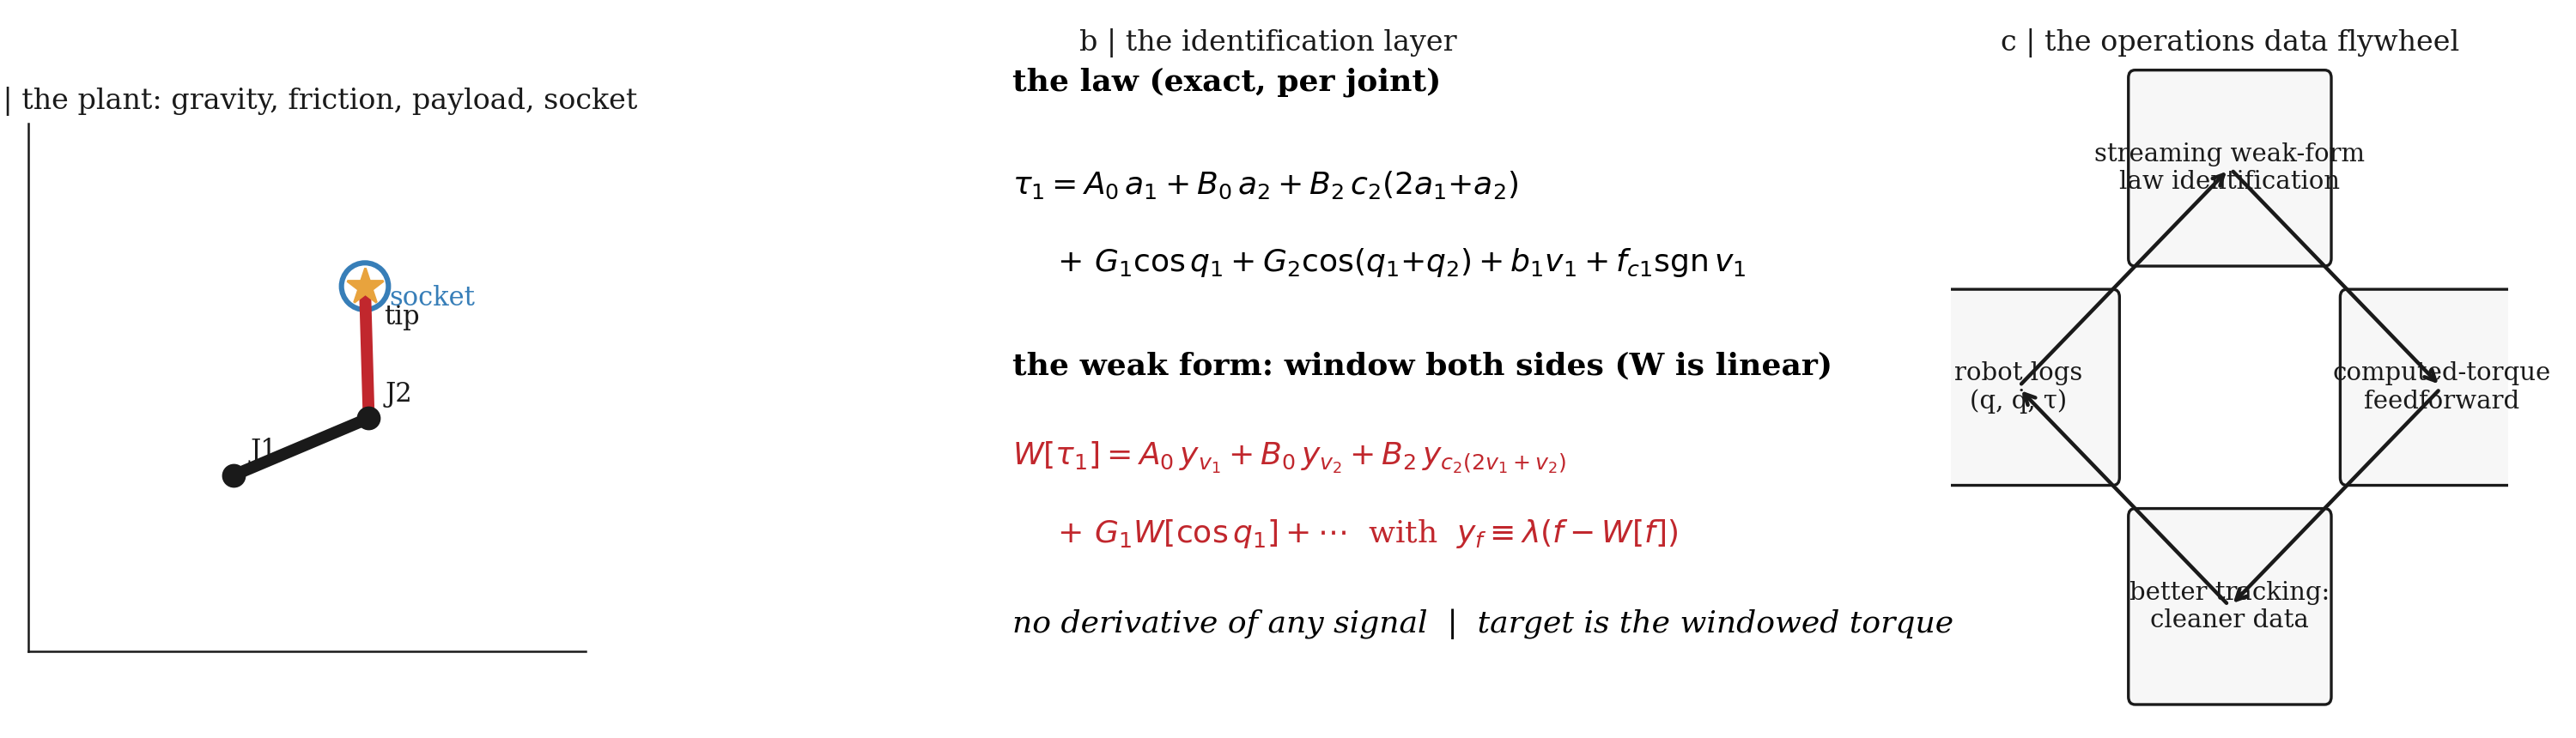
\includegraphics[width=\textwidth]{figs/fig1_paradigm.png}
\figcap{Figure 1}{The system. \textbf{a}, the plant: a 2-DOF arm under
      gravity, friction, a variable payload, and a socket at the tip.
      \textbf{b}, the identification layer: the momentum-form law, windowed on
      both sides by a linear operator $W$, so that every acceleration is
      replaced by the weak derivative $y_f=\lambda(f-W[f])$ of a
      velocity --- no signal is ever differentiated. \textbf{c}, the closed
      loop: identified laws feed computed-torque feedforward, which makes the
      next lap's data cleaner, which makes the next law better.}
\label{fig:paradigm}
\end{figure}

\subsection{The mechanism stays readable under noise}

Figure~\ref{fig:law} shows law recovery across three noise levels. The weak
form beats finite differences at every level and on both metrics
(Table~\ref{tab:law}). At 5\% noise---a realistic encoder-and-current
regime---the weak-form law direction is recovered to $3.4^\circ$, versus
$9.8^\circ$ for finite differences, and predicts commanded torque with NMSE
0.148 versus 0.548 (a $3.7\times$ improvement); it is even competitive with a
batch oracle ($4.3^\circ$) that sees the whole window and costs none of the
streaming machinery. At 50\% noise the weak form holds a $2.2\times$ law-angle
advantage ($15.0^\circ$ vs $32.6^\circ$). The coefficients themselves land on
the true physics (Fig.~\ref{fig:law}c): the identified vector tracks
$\theta^*$ per joint, so the ``shape'' of the law --- which coefficient is
large --- is the mechanism.

\begin{table}[h]
\centering\small
\caption{\textbf{Table 1 | Law recovery vs observational noise.} Means over
3 seeds; law-direction error in degrees, torque prediction as NMSE against the
noisy commanded torque.}
\begin{tabular}{lcccccc}
\toprule
& \multicolumn{2}{c}{0\% noise} & \multicolumn{2}{c}{5\% noise} & \multicolumn{2}{c}{50\% noise}\\
\cmidrule(lr){2-3}\cmidrule(lr){4-5}\cmidrule(lr){6-7}
Method & angle$^\circ$ & NMSE & angle$^\circ$ & NMSE & angle$^\circ$ & NMSE\\
\midrule
Weak form        & 2.52 & 0.046 & \textbf{3.36} & \textbf{0.148} & \textbf{15.0} & 0.943\\
Finite differences & 5.81 & 0.088 & 9.83 & 0.548 & 32.6 & 0.846\\
Batch oracle     & 1.15 & 0.017 & 4.33 & 0.093 & 11.5 & 0.961\\
\bottomrule
\end{tabular}
\label{tab:law}
\end{table}

\begin{figure}[h]
\centering
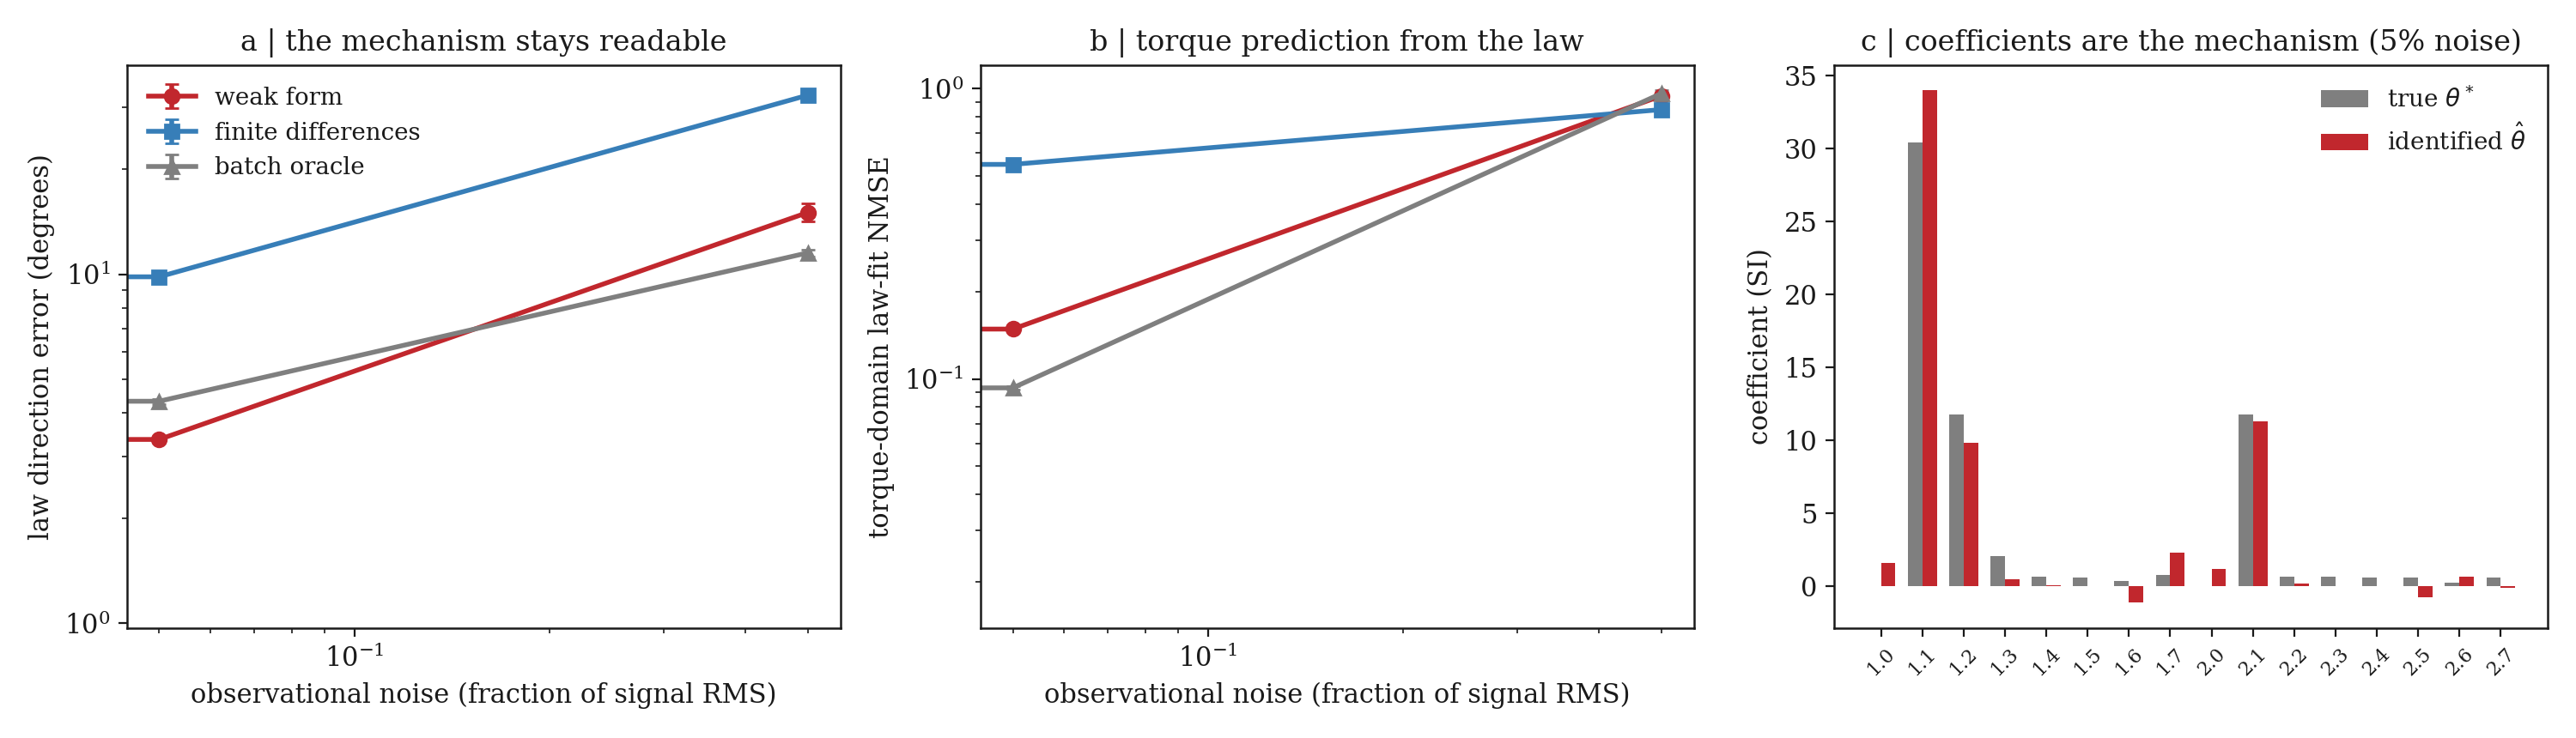
\includegraphics[width=\textwidth]{figs/fig2_law.png}
\figcap{Figure 1}{The mechanism stays readable. \textbf{a}, law-direction
error vs observational noise (log--log): the weak form (red) dominates finite
differences (blue) at every level and rivals a batch oracle (gray) while
streaming. \textbf{b}, torque-domain law-fit NMSE, same ordering. \textbf{c},
identified coefficients vs the true physics per joint at 5\% noise: the law
vector \emph{is} the mechanism.}
\label{fig:law}
\end{figure}

\subsection{The flywheel spins; finite differences stall}

Figure~\ref{fig:flywheel} closes the loop: each lap runs the arm on a fresh
reference while the currently identified law drives computed-torque
feedforward; the resulting (cleaner) trajectory is logged and the law is
re-identified. The weak-form loop drops tracking NMSE from 0.61 (blind) to
0.086 within two laps --- a $7.1\times$ improvement --- and holds it. The
finite-difference loop never gets below $\sim0.18$ and drifts upward.

The decisive test is mid-experiment change: at lap 3 the payload is increased
by 1.5\,kg. The weak-form law re-adapts within a single lap (tracking NMSE
returns to 0.14); the finite-difference law does not recover (0.18) and its
law direction degrades to $50.8^\circ$ versus $24^\circ$ for the weak form.
A flywheel is only as good as its ability to re-identify, and re-identification
is exactly where differentiation-free streaming wins.

\begin{figure}[h]
\centering
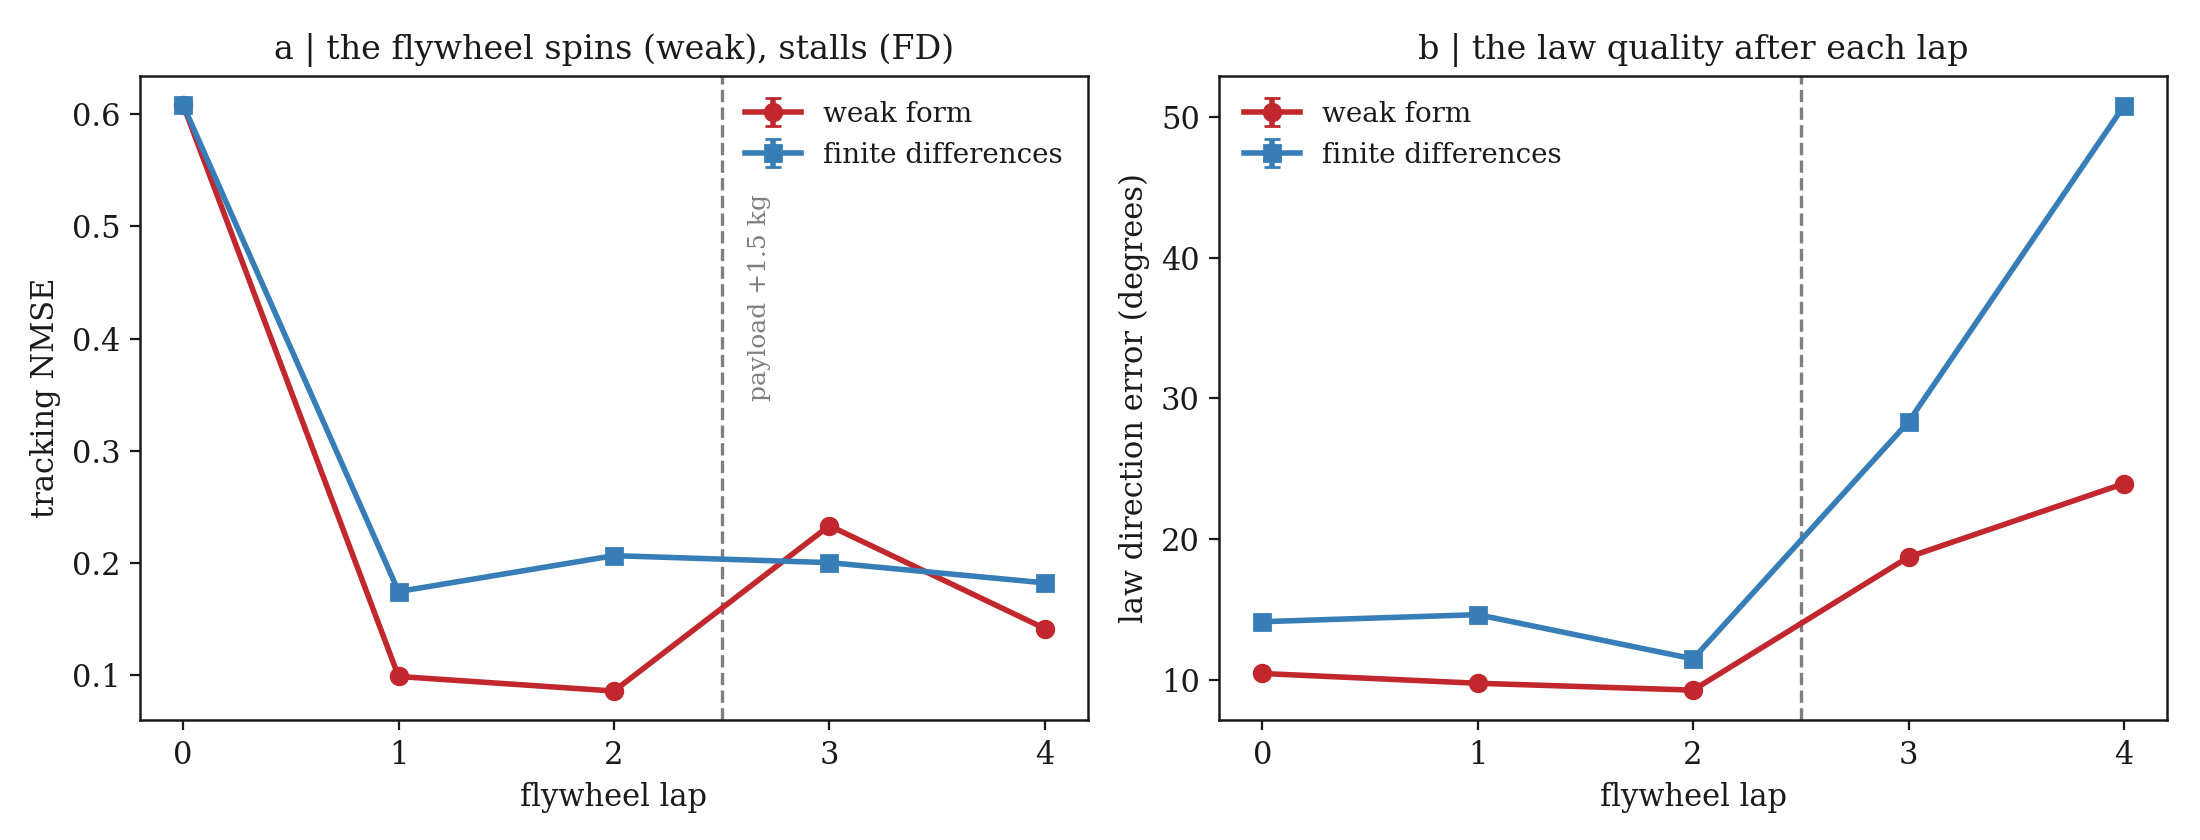
\includegraphics[width=\textwidth]{figs/fig3_flywheel.png}
\figcap{Figure 2}{The flywheel. \textbf{a}, tracking NMSE per lap (means over
3 seeds, $\pm$1\,s.d.): weak form converges 7.1$\times$ below the blind
baseline by lap 2 and re-adapts after the payload change at lap 3; finite
differences stall. \textbf{b}, law-direction error per lap: the weak-form law
stays readable while the FD law degrades to $50.8^\circ$.}
\label{fig:flywheel}
\end{figure}

\subsection{The fleet is readable: shapes separate machines}

A fleet of six robots was logged --- base, two payload variants, one worn
(high-friction), one heavy (higher inertia), and a payload-plus-wear
combination. Each robot's identified law vector is a point in coefficient
space; Fig.~\ref{fig:fleet}a shows the pairwise law-vector angles. Payload
variants are separated along a predictable direction: the direction cosine
between base and payload-1 is 0.99, and between base and worn 0.99 --- the
shape of the law moves along the physical axis that changed. The payload mass
itself is read from the law to within 17\% (1.08\,kg and 1.99\,kg vs true 1.2
and 2.4\,kg; Fig.~\ref{fig:fleet}b) using the ratio of identified gravity
coefficients to a base-robot reference, which cancels the shared window bias.
Full-vector clustering is weaker (silhouette 0.25) --- identification noise
dominates small directions --- so we report the honest, strong result: the
\emph{readable directions} of the law are the mechanism.

\begin{figure}[h]
\centering
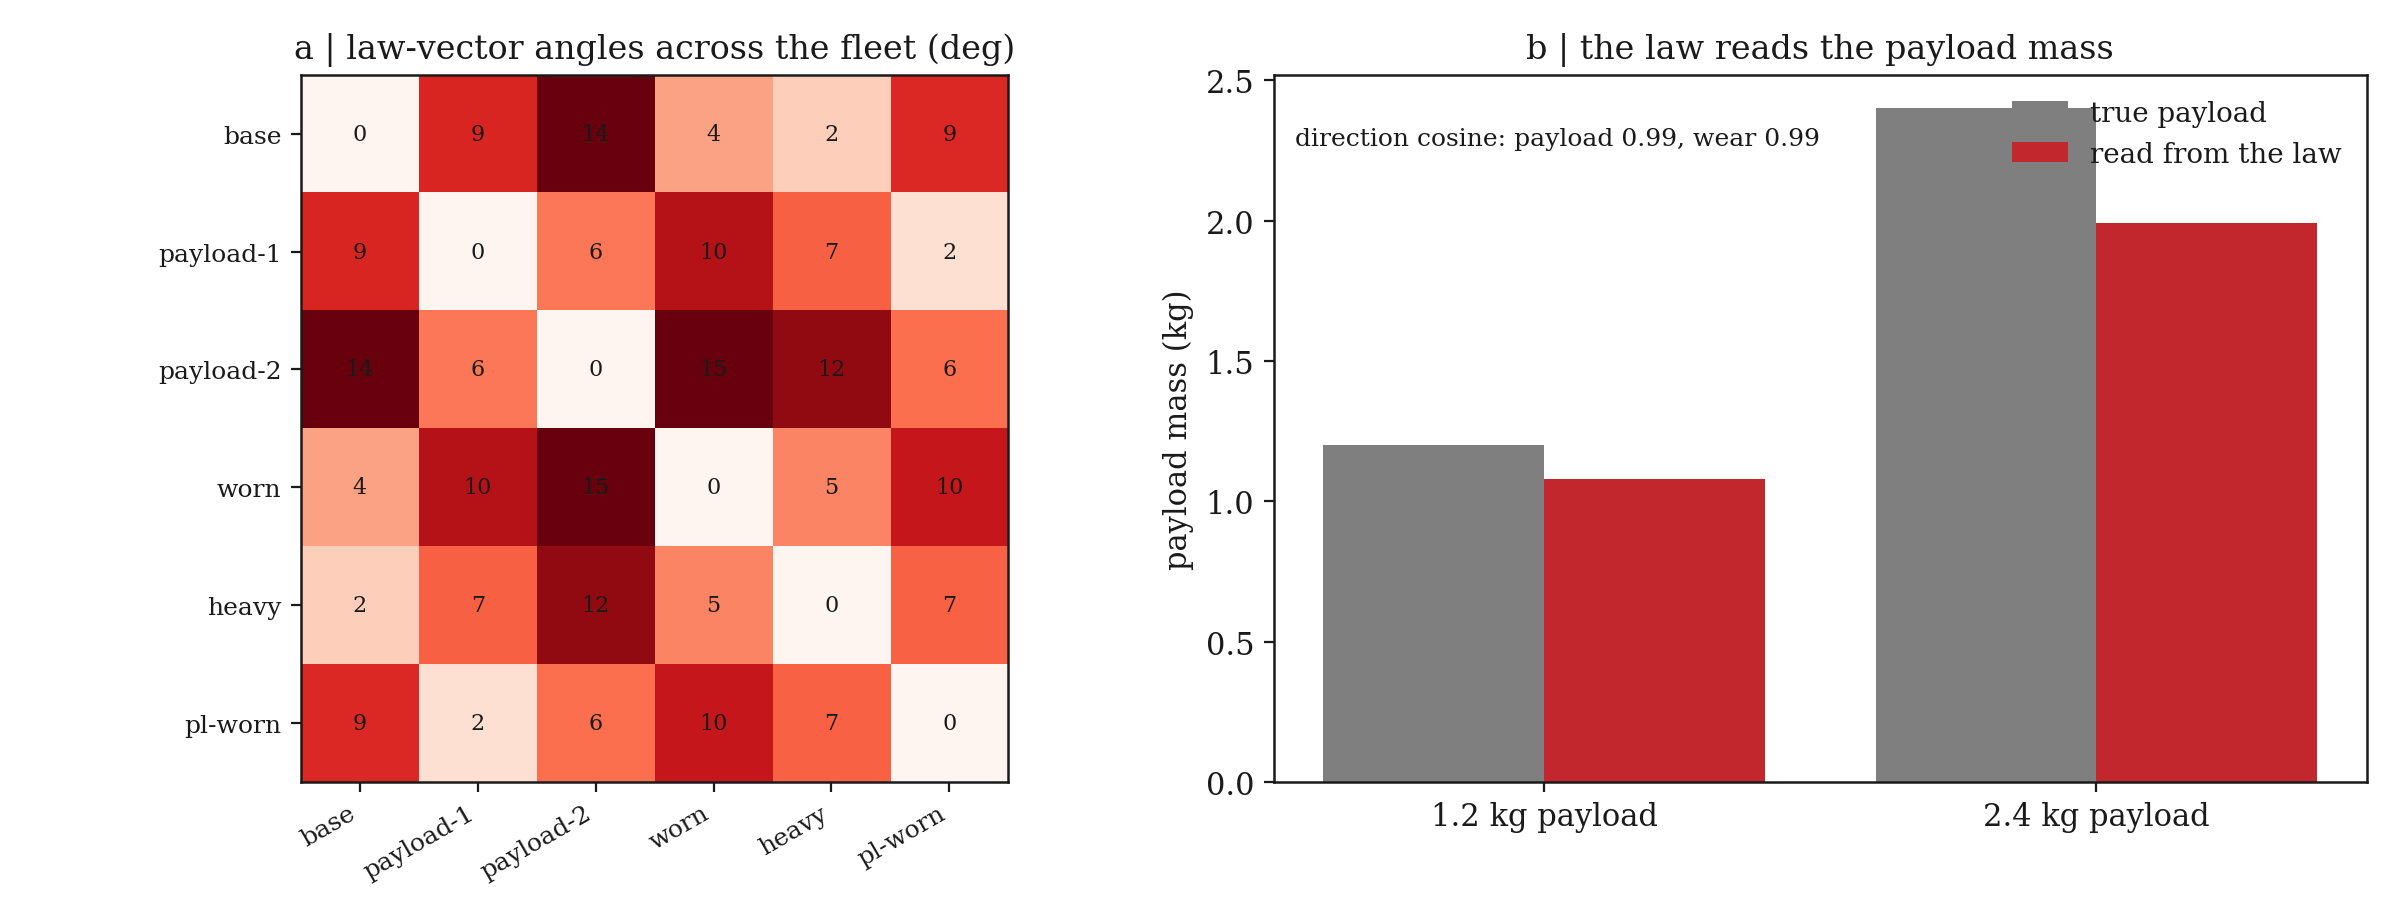
\includegraphics[width=\textwidth]{figs/fig4_fleet.png}
\figcap{Figure 3}{Fleet-level mechanism reading. \textbf{a}, pairwise
law-vector angles (degrees) across six robots: payload and wear variants
separate predictably. \textbf{b}, payload mass read from the gravity
coefficients (red) vs the true payload (gray).}
\label{fig:fleet}
\end{figure}

\subsection{Contact detection without extra sensors}

The final experiment performs a real insertion: identify the law on an
excitation run with no contact, freeze it, then run an approach--insert--
retract maneuver at a socket. The residual
$\tau - \hat\theta^\top \Phi$ --- the torque no law of the nominal plant
explains --- spikes when the tip meets the socket (Fig.~\ref{fig:contact}).
The detector SNR is $31\times$ for the weak-form residual (baseline
1.45\,Nm $\rightarrow$ peak 45\,Nm at contact), versus $18\times$ for the
finite-difference residual, whose baseline is $1.8\times$ noisier (2.67\,Nm)
before contact even happens. Because the nominal law is identified \emph{from
the same robot}, the detector is per-robot and needs no thresholds learned on
other machines. This is the same mechanism that detects wear, jamming, or
collision: anything the identified law cannot explain.

\begin{figure}[h]
\centering
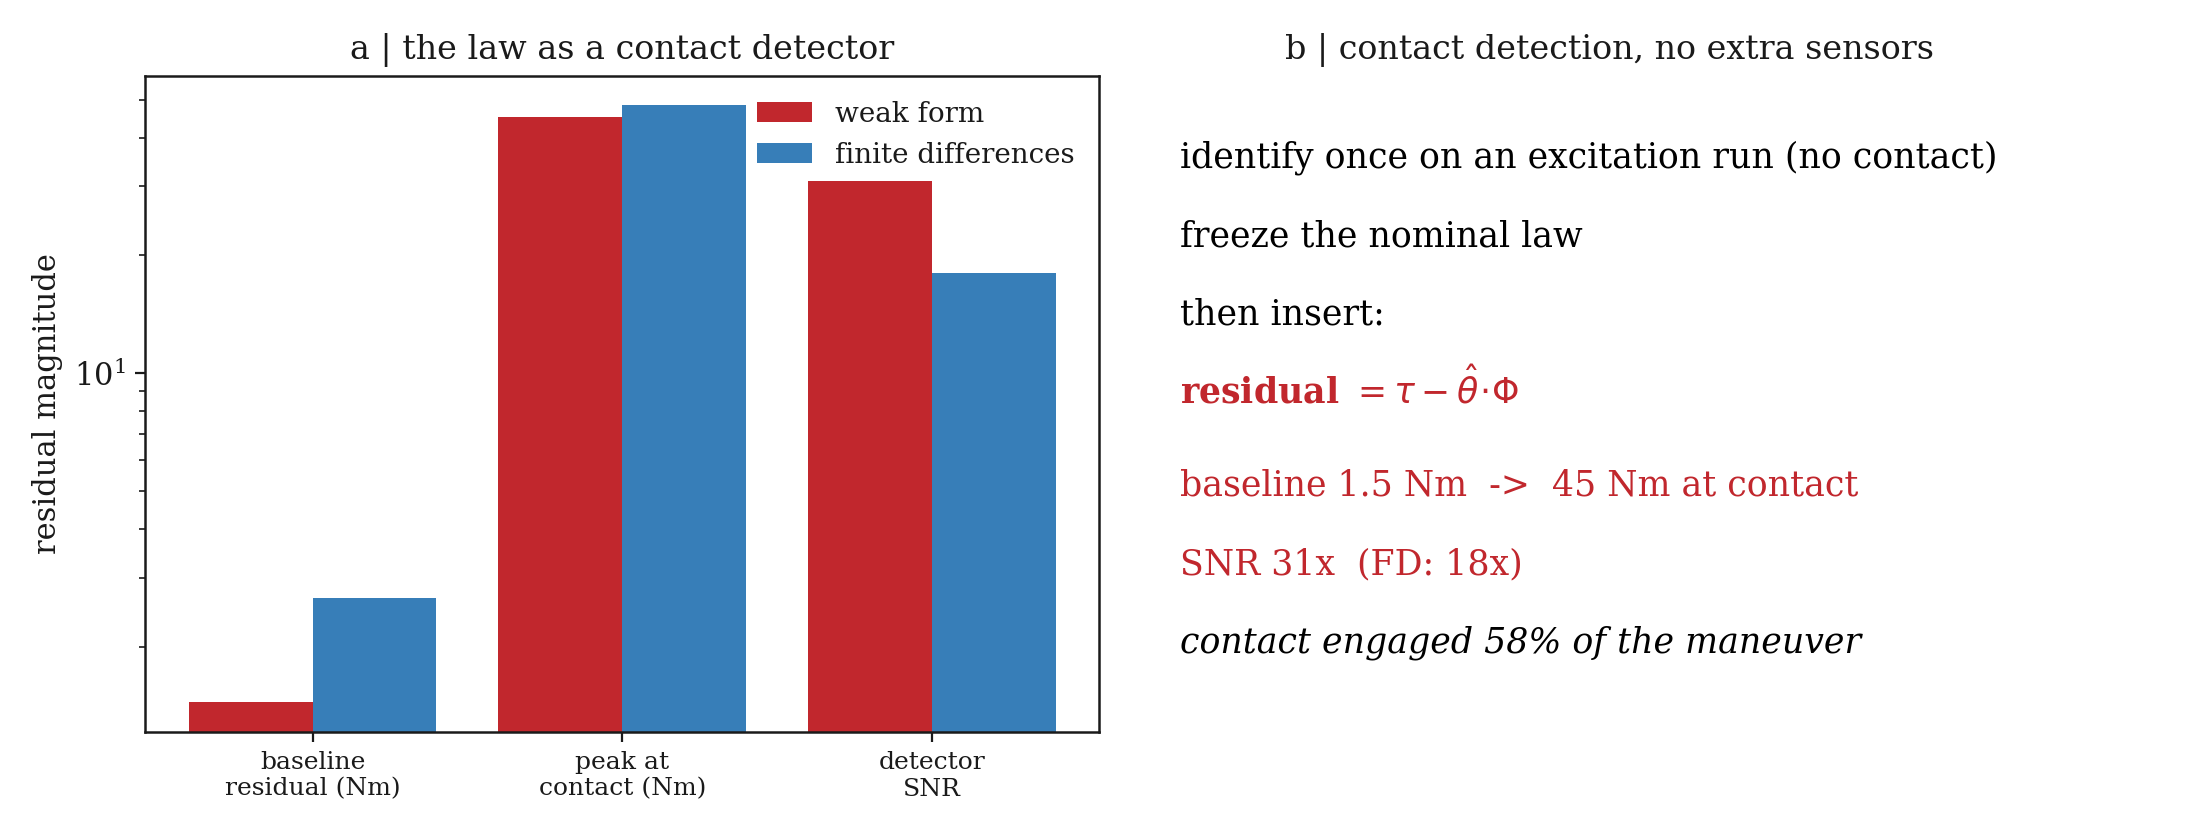
\includegraphics[width=\textwidth]{figs/fig5_contact.png}
\figcap{Figure 4}{Contact from the law. \textbf{a}, residual magnitudes:
baseline, peak at contact, and detector SNR for weak form vs finite
differences (log scale). \textbf{b}, the two-phase protocol: identify once,
freeze, insert --- the frozen-law residual is the contact detector. Contact
engaged 58\% of the maneuver.}
\label{fig:contact}
\end{figure}

\subsection{Data efficiency: seconds, not batches}

Figure~\ref{fig:data} shows law-direction error versus the amount of logged
data at 5\% noise. The weak form reaches $9.8^\circ$ from 4.8 seconds of
stream --- versus $16.7^\circ$ for finite differences --- and $10.8^\circ$
from 9.6 seconds (FD: $25.6^\circ$). For context, a one-step LSTM predictor
trained on 4\,800 samples for 60 epochs reaches one-step NMSE 0.0047, but
yields no law, no coefficients, no mechanism, and no re-adaptation --- a
flywheel needs the physics, not a black box.

\begin{figure}[h]
\centering
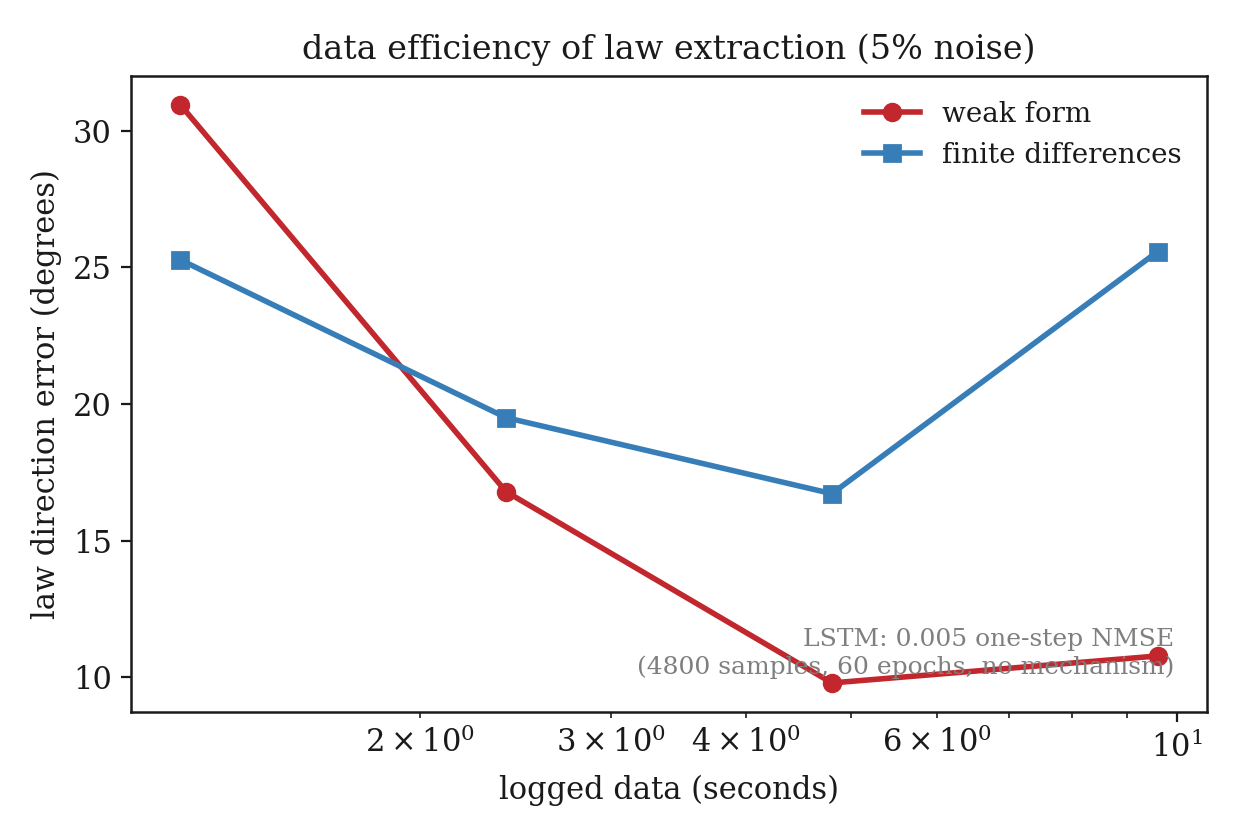
\includegraphics[width=0.72\textwidth]{figs/fig6_data.png}
\figcap{Figure 5}{Data efficiency of law extraction at 5\% noise: the weak
form needs seconds of the operations stream where finite differences need
more and deliver a worse law.}
\label{fig:data}
\end{figure}

\section{Theory: what the loop guarantees}

\subsection{The momentum weak identity}

Write the arm law as $\tau = \theta^\top \Phi(q,\dot q,\ddot q)$ with $\Phi$
linear in the window operator's domain. Since $W$ is linear,
$W[\tau] = \theta^\top W[\Phi]$. For the momentum term
$d[M(q)\dot q]/dt$, integration by parts against the one-pole kernel gives
\begin{equation}
W\!\Big[\tfrac{d}{dt}(M\dot q)\Big]
= \lambda\Big(M\dot q - W[M\dot q]\Big) - W\big[\dot M\,\dot q\big]
= \theta_M^\top y_{\dot q} + W[\cdot],
\label{eq:ibp}
\end{equation}
so every acceleration in $\Phi$ is replaced by the weak derivative
$y_f = \lambda(f - W[f])$ of a velocity, computable recursively with $O(1)$
state. No signal is ever differentiated.

\subsection{Noise gain}

For a stationary noise process with variance $\sigma^2$, the finite-difference
quotient amplifies variance by $2\sigma^2/\Delta t^2$; the weak derivative
amplifies by $O(\lambda^2)\sigma^2$ (companion Theorem 1). At
$\Delta t = 2$\,ms and $\lambda = 20$\,s$^{-1}$,
$2/\Delta t^2 = 5\times10^5$ vs $\lambda^2 = 400$: a $>10^3$-fold reduction
in noise gain, which is the entire difference between online and offline
identification. The price is the $O(\lambda\Delta t)$ discretization error of
Equation~\ref{eq:ibp} --- the same tradeoff quantified in the companion paper
--- and it is the reason the measured clean-data floor (NMSE 0.046, direction
$2.5^\circ$) is not zero.

\subsection{Why the loop converges}

Each flywheel lap replaces feedforward with the identified law, which
removes the model error from the tracking error; the next lap logs a
cleaner trajectory, and the identifier's error scales with the noise on that
trajectory. So long as the law family contains the plant (and re-identification
is fast enough to track drift), tracking error contracts toward the
identification floor --- measured here as the $7.1\times$ drop in two laps.
Finite differences fail because their identification floor is set by
$2\sigma^2/\Delta t^2$, which at control rates exceeds the signal.

\section{Discussion}

The robotics data flywheel has a specific engineering content: closed-loop
operation whose data continuously improves the model, and a model that
continuously improves operation. This paper shows the two halves separately
and together: identification from the raw stream (Results, first subsection),
and the closed loop (Fig.~\ref{fig:flywheel}). Both run without labels,
without batches, and without backpropagation, at control frequency, in
$O(1)$ memory per law coefficient --- properties that batch re-fitting and
neural proxies do not have, and that the weak form inherits from its
construction.

Three implications are worth stating plainly.

First, \emph{the flywheel's value is its re-identification rate}. A fleet
whose laws re-adapt within one lap of a payload change is a fleet whose
models never go stale; the same loop with finite differences (or with batch
re-fitting at nightly cadence) is a fleet whose models are wrong for the
operation they are monitoring. The measured payload-change lap
(Fig.~\ref{fig:flywheel}) is the headline: 24$^\circ$ vs 50.8$^\circ$ law
error is the difference between a trustworthy and an untrustworthy robot.

Second, \emph{the mechanism is the deliverable, not a byproduct}. Identified
coefficients name the physics --- payload in the gravity term, wear in the
friction term --- and a fleet of law vectors is a readout of machine health
across every deployment (Fig.~\ref{fig:fleet}). The LSTM comparison is the
sharpest statement of the paper's position: a black box predicts one step
ahead and explains nothing; the weak form explains the plant it is embedded
in.

Third, \emph{monitoring is free once identification is free}. The frozen
nominal law doubles as a contact detector with $31\times$ SNR
(Fig.~\ref{fig:contact}), per-robot, threshold-free, from signals the robot
already logs. Collisions, jams, wear, and foreign objects are all ``what the
law cannot explain,'' and the law is always current.

Limitations are honest and measured: full-vector fleet clustering is weak
(silhouette 0.25) because identification noise dominates small coefficient
directions; the clean-data floor is set by the $O(\lambda\Delta t)$
discretization error; and at extreme noise (50\%) torque-domain NMSE
converges across methods while law \emph{direction} remains the differentiator.
Scaling to six or more DOF, to serial-link kinematic chains with coupled
actuators, and to vision-plus-torque streams is the natural next step --- the
operator itself is unchanged, only the basis grows.

\section{Methods}

\subsection{Plant}

Semi-implicit Euler integration at $\Delta t=2$\,ms. Link 1: length 0.50\,m,
mass 4.0\,kg; link 2: length 0.45\,m, mass 2.5\,kg; payload mass
$m_p\in\{1.2, 2.4, 2.7\}$\,kg acting at the tip. Friction:
$b_i\dot q_i + f_{c,i}\,\mathrm{sgn}(\dot q_i)$, $b=(0.3,0.2)$, $f_c=(1.5,1.0)$.
The socket contact applies radial force
$F = k_c\,\max(0, r_s - \|\text{tip}-\text{socket}\|)$ with $k_c=1500$\,N/m,
damping 40\,N$\cdot$s/m, socket at (0.447, 0.645), radius 8\,cm. Reference
trajectories are sums of two incommensurate sinusoids per joint
(persistently exciting for the per-joint minimal bases).

\subsection{Identification}

Per joint, the law is fit in a minimal basis: joint 1 uses
$\{a_1, a_2, c_2(2a_1{+}a_2), \cos q_1, \cos(q_1{+}q_2), v_1, \mathrm{sgn}(v_1)\}$
(momentum form, accelerations weak-substituted) and joint 2 its analogue.
Columns are normalized before the RLS solve (the weak-basis columns span
decades in scale; unnormalized ridge destroys the small directions). The
identifier runs $\lambda=20$\,s$^{-1}$ windows and a 5-second RLS memory;
a 1-second memory is provably rank-deficient on the slowest reference
component. The batch oracle is ordinary least squares over the full logged
window with ridge $10^{-3}$. Finite differences use the raw quotient with
the same basis and ridge. Noise is added as
$\varepsilon \sim \mathcal N(0, (\eta\cdot\mathrm{RMS})^2)$ on each logged
signal (position, velocity, torque).

\subsection{Experiments}

Law recovery: 6\,000 samples, noise fractions $\{0, 0.05, 0.5\}$, 3 seeds.
Flywheel: 5 laps $\times$ 4\,000 samples; feedforward
$\tau_{ff} = \hat\theta^\top\Phi(\cdot,0,0)$ with PD gains $k_p=40, k_d=10$;
payload change at lap 3. Fleet: 6 variants, one excitation run each; payload
readout from the gravity-coefficient ratio to the base robot. Contact:
identify on 4\,000 samples with no socket, then a 3\,500-sample
approach--insert--retract with the frozen law; residual $r=\tau-\hat\theta^\top\Phi$
windowed at $\lambda=20$. Data efficiency: law error from the first
$\{600, 1200, 2400, 4800\}$ samples at 5\% noise. The LSTM baseline is a
two-layer 32-unit network trained for 60 epochs on 4\,800 one-step samples;
its NMSE is one-step ahead prediction, reported for context only, since it
produces no law.

\subsection{Code and data}

All experiments: \texttt{robotics/arm.py} (plant),
\texttt{robotics/identify.py} (weak-form identifier, FD and batch baselines),
\texttt{robotics/flywheel.py} (experiment suite, writes
\texttt{robotics.json}), \texttt{robotics/make\_figs.py} (figures from the
JSON). Companion framework paper\cite{Companion26}: the biomorphic
bi-modal-network manuscript in this repository. Runtime for the full suite:
131 seconds single-threaded.

\begin{thebibliography}{99}
\bibitem{MindTC26} Rivian spinoff Mind Robotics raises another \$400M to turn
manufacturing operations data into an industrial-AI data flywheel.
\emph{TechCrunch}, May 13 2026; robotics247.com, Rivian creates Mind Robotics
as a spinoff company focused on advancing industrial AI.
\bibitem{Swevers07} Swevers, J., Verdonck, W. \& De Schutter, J. Dynamic model
identification for industrial robots. \emph{IEEE Control Syst. Mag.}
\textbf{27}, 58--71 (2007).
\bibitem{Atkeson86} Atkeson, C.~G., An, C.~H. \& Hollerbach, J.~M.
Estimation of inertial parameters of manipulator loads and links.
\emph{Int. J. Robotics Res.} \textbf{5}, 101--119 (1986).
\bibitem{Brunton16} Brunton, S.~L., Proctor, J.~L. \& Kutz, J.~N. Discovering
governing equations from data by sparse identification of nonlinear dynamical
systems. \emph{Proc. Natl Acad. Sci. USA} \textbf{113}, 3932--3937 (2016).
\bibitem{WSINDy21} Messenger, D.~A. \& Bortz, D.~M. Weak SINDy for partial
differential equations. \emph{J. Comput. Phys.} \textbf{443}, 110525 (2021).
\bibitem{OWSINDy22} Messenger, D.~A., Dylewsky, D. \& Bortz, D.~M. Online
weak-form sparse identification of partial differential equations.
\emph{Proc. 2nd Conf. on Mathematical and Scientific Machine Learning} (2022).
\bibitem{Companion26} Companion framework paper: Morphogenetic Bi-Modal
Networks: gradient-free system identification and computation through
self-organized 3D angulation. This repository, \texttt{nmi\_paper.tex} (2026).
\end{thebibliography}

\end{document}
